\documentclass[10pt,twocolumn,letterpaper]{article}

\usepackage{cvpr}
\usepackage{times}
\usepackage{epsfig}
\usepackage{graphicx}
\usepackage{amsmath}
\usepackage{amssymb}

% Include other packages here, before hyperref.

% If you comment hyperref and then uncomment it, you should delete
% egpaper.aux before re-running latex.  (Or just hit 'q' on the first latex
% run, let it finish, and you should be clear).
\usepackage[breaklinks=true,bookmarks=false]{hyperref}

\cvprfinalcopy % *** Uncomment this line for the final submission

\def\cvprPaperID{****} % *** Enter the CVPR Paper ID here
\def\httilde{\mbox{\tt\raisebox{-.5ex}{\symbol{126}}}}

% Pages are numbered in submission mode, and unnumbered in camera-ready
%\ifcvprfinal\pagestyle{empty}\fi
\setcounter{page}{4321}
\begin{document}

%%%%%%%%% TITLE
\title{Measurements with Cell Phones and Credit Cards}

\author{Chase Lambert\\
MIT\\
Cambridge, MA\\
{\tt\small lambertc@mit.edu}
% For a paper whose authors are all at the same institution,
% omit the following lines up until the closing ``}''.
% Additional authors and addresses can be added with ``\and'',
% just like the second author.
% To save space, use either the email address or home page, not both
\and
Akhil Raju\\
MIT\\
Cambridge, MA\\
{\tt\small araju@mit.edu}
}

\maketitle
%\thispagestyle{empty}

%%%%%%%%% ABSTRACT
\begin{abstract}
We propose a method to find the dimensions of objects in an environment using a cell phone and a credit card. The credit card is automatically found in the image, mainly using convolutions and the distance transform, and the user is then given the chance to measure objects. Our approach works well under reasonable lighting conditions when the phone is about 30 cm away from the object, but degrades in quality as the card gets smaller in the image.
\end{abstract}

%%%%%%%%% BODY TEXT
\section{Introduction}

Humans have used rulers for over four Millennia. But while measurements have gotten more accurate, they haven’t become much more convenient. In this paper, we describe a way in which almost everyone can have access to a quick and accurate ruler at any point in time. The idea is to use two items most people carry - a credit or debit card, and a camera phone. The user places their card next to the object they want to measure, and takes a picture of it. The user then selects which region of the image that they want to measure, and they get an answer. The phone does this by finding the accurate location of the card in the image, and calculating the distance by using the known size of a credit card.

\begin{figure}[t]
\begin{center}
   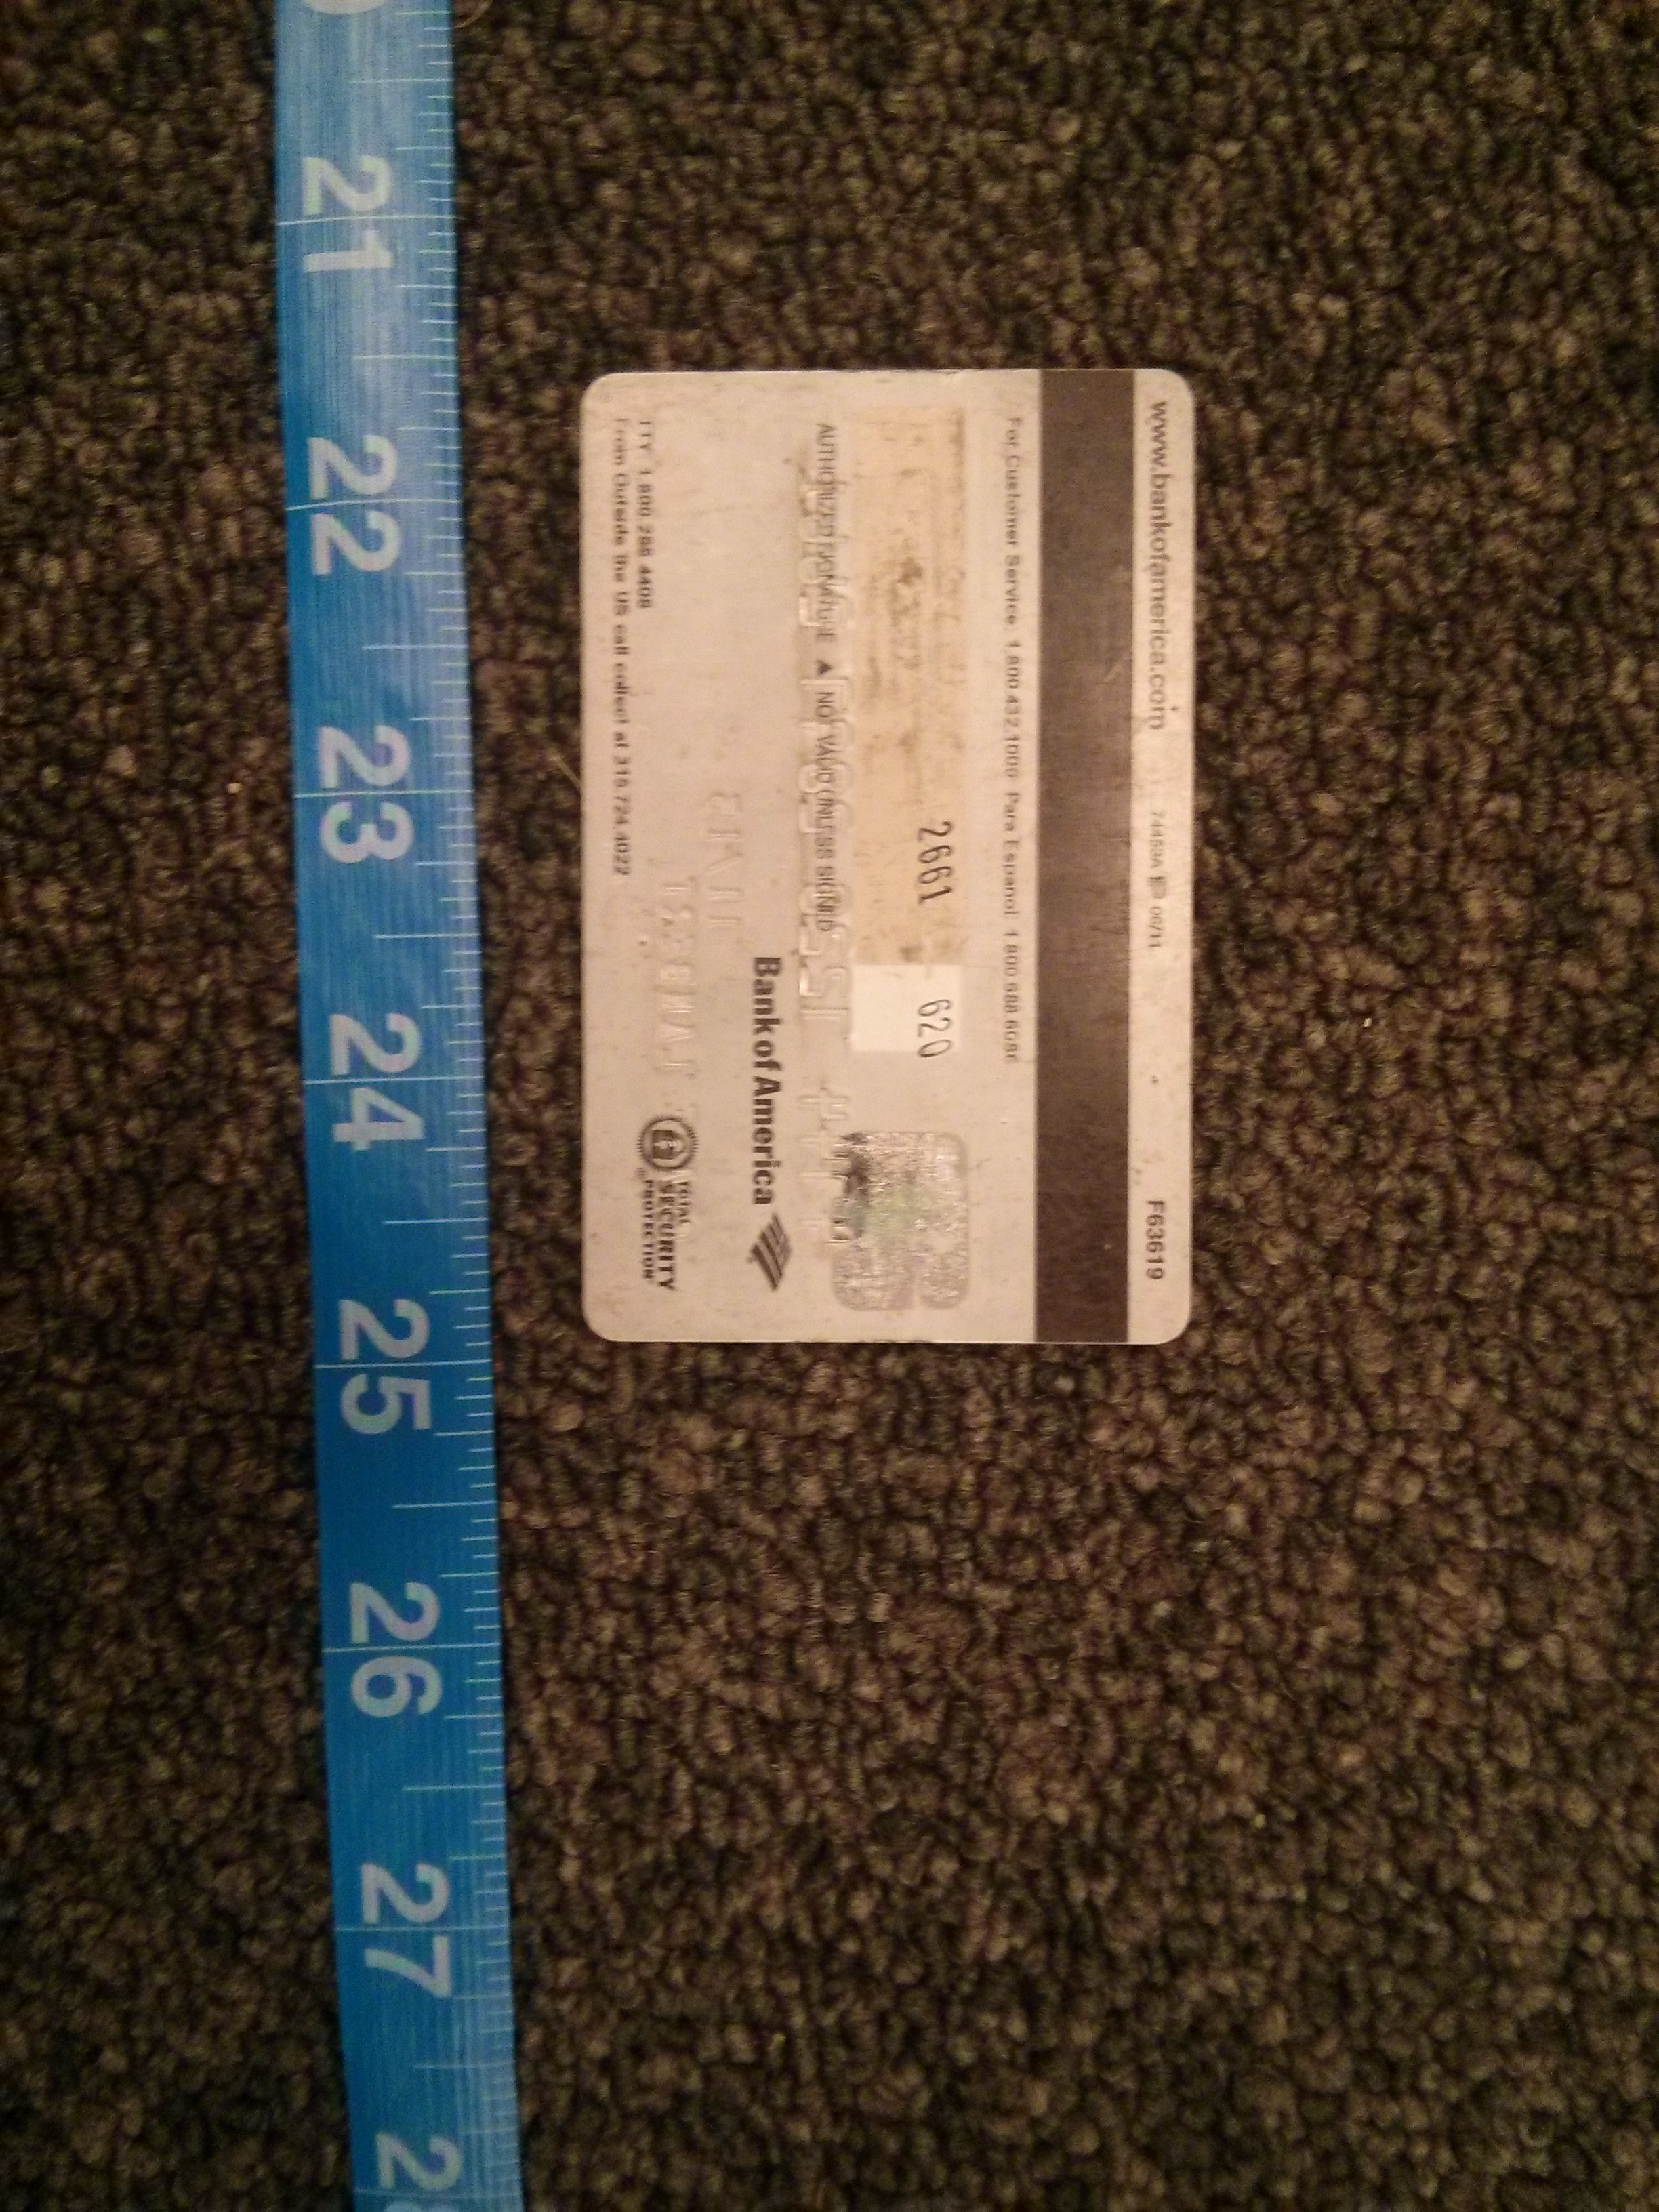
\includegraphics[width=0.8\linewidth]{one}
\end{center}
   \caption{something}
\label{fig:first}
\end{figure}


%-------------------------------------------------------------------------
\subsection{Related Work}

On the surface, some fig \ref{fig:first} it seems that there’s been an immense amount of research that’s been done on the same subject that we are trying to tackle - object recognition. Papers have been published recognizing not just one object, but many \cite{ObjectDetection}. And face recognition is highly accurate \cite{FaceDetection}. But our requirements are slightly different - we need a near perfect bounding box. The vast majority of research that is done on object recognition only needs a somewhat accurate box, because their main concern is reducing false categorizations in the large array of situations they are trying to study. We, instead, have a very standard set of images to search through, but require a highly accurate bounding box such that we can give good measurements.

As for measuring objects using a phone, the popular applications require the user to manually specify where reference objects are. The Android application called PhotoRuler \cite{PhotoRuler} requires the user to take a picture, and then draw arrows around the reference object (like a credit card) and around the object to be measured (todo fig. PhotoRuler). There is a similar iPhone application \cite{RulerPhone}, but it requires the user to move the camera around to overlay a reference card that is displayed along with the video feed. A different approach is just a ruler displayed on a phone \cite{SmartRuler}. But this rough approach at solving the more general problem just pushes towards the need for a better portable ruler.

Other approaches to finding measurements are physical devices. While normal sized rulers are too large to carry around, CardStick is a “durable vinyl ruler decal that fits any credit, debit, or other card.” \cite{CardStick}. This may work well for objects that are smaller than a credit card, but no larger. And even with this limitation, users are impressed - the product has nearly five stars on Amazon.

%------------------------------------------------------------------------
\section{Methods and Approaches}
Our program allows the user to measure objects in an image through two steps. First, the program identifies the credit card in the image, which gives objects in the image a sense of scale. Second, the user denotes the object he or she wants to measure. 

There are four different, but related, approaches we use in solving the problem of credit card detection. The first approach uses edge detection and Chamfer matching to find a credit card in a plain background, and then pinpoints the card in a more complex scene using matched image features. The second approach simply relies on Chamfer matching to find a credit card in any image. \cite{chamfer}. The third approach finds the region in the scene image which best matches the distance transform of a template card. The fourth utilizes SketchTokens to help find edges and complete Chamfer matching. \cite{SketchTokens}. 

Once the credit card is identified in the scene, the user is able to drag a line across the image, and the program outputs the length of that line. As per our assumptions, the object the user is trying to measure is approximately the same distance from the camera as the credit card. Almost all credit cards have standardized dimensions for the card (54 mm X 86 mm) and the magnetic strip (9.5 mm X 86 mm, 5.5 mm from the top of the card). The credit card detection supplies a conversion from pixel length to centimeters since we know the dimensions of the card in the image and in the physical world, and that conversion is used to convert the pixel length of the user’s line to a physical distance in centimeters. 

	The algorithms are implemented in Matlab, which provides many useful and necessary functions for different aspects of the approaches, like edge detection, extracting SIFT or SURF features, and two dimensional convolutions.  

\subsection{Assumptions}

	We rely on several key assumptions to make the measurement process fast and possible:


- The plane the credit card rests on is perpendicular to the camera axis.

- The object the user is trying to measure lies on the same plane as the credit card (same distance from the camera). 

- The magnetic strip of the credit card runs horizontally across the image.


The first two assumptions make the measurements more accurate and easy to infer from the image. The final assumption simplifies the process of finding the credit card, making the credit card detection step run faster for testing purposes. The first approach below actually handles different card orientations, and the second and third approaches can easily expand to handle different orientations. 

\subsection{Chamfer Matching and Image Features}
\subsubsection{Algorithm}
This approach first requires the user to take a picture of their card in a plain background, wherein the algorithm finds the card using Chamfer distances \cite{chamfer}. Since the algorithm is edge based, we require that the user take a picture of the back of the credit card, which offers more defined edges due to the black magnetic strip found on the back of cards. The algorithm first uses a Canny edge detector to extract the edges of the image. Our experiments show that the Canny edge detection algorithm works better for this than other edge detection algorithms, like the Sobel edge detection algorithm \cite{canny}. Then, the distance transform of the image is calculated, which allows for the Chamfer distances to be calculated more efficiently. Iteratively, different edge templates of a credit card at different scales are convolved with the distance transform of the image, yielding the Chamfer distances. After normalizing for scale, the lowest Chamfer distance denotes where the card is in the image.

Once the card has been identified in the image, the features of the image are extracted. The user takes a second image of a scene in which he or she wants to measure some object. The same credit card is present in this second image. The algorithm looks for matching feature points between the credit card image and the scene image, and using RANSAC, it finds the credit card in the image and computes the homography from the card in the plain image to the one in the scene image \cite{ransac}. We experimented with extracting different sets of features, including SIFT and SURF features, and SURF features yielded more success in finding the credit card \cite{sift} \cite{surf}. 

\subsubsection{Stengths}
	This approach is designed to find the card in various orientations in the scene image, and it does so well in scenes that are not too large or complex. Chamfer matching provides a robust method of finding the credit card in a plain background, even in a range of lighting conditions. Given that the card is a significant portion of the scene, the algorithm can successfully use SURF features to find the card in the scene, regardless of its homography. 
	
\subsubsection{Weaknesses}
	This approach breaks down in scenes in which the card is a small portion of the image. In such scenes, the card is often more blurry than the card in the reference image (with the plain background) because the image simply devotes less resolution to describing the card. While image features like SIFT and SURF are said to be scale-invariant, they are not blur-invariant, so the SIFT and SURF descriptors fail to find matches between the large, clear reference card and the small, blurry card in the scene. TODO: maybe cite scale invariant stuff. Chase maybe can describe this approach better. 
	
\subsection{Only Chamfer Matching}
The second approach only requires the user take the image of the scene. This algorithm first shrinks the image, allowing for faster runtimes and cleaner edge detection. TODO: maybe include some evidence of this. Following the resizing, the algorithm goes through the same process as the first approach: it finds the minimum Chamfer distance by convolving credit card edge-templates at different scales with the distance transform of the scene. The location and scale of the template that yields the minimum Chamfer distance describes the best guess of where the credit card is in the image. 
	Instead of using all the edges of the credit card, however, this approach only relies on the edges of the magnetic strip, as those edges are most often the strongest edges in the scene. Thus, using a more discriminatory edge detector allows the algorithm to easily find the credit card because the edge detector extracts very few edges other than those of the magnetic strip.

\subsubsection{Strengths}
	Somewhat surprisingly, the pure Chamfer matching approach works reliably and quickly in well-lit conditions. TODO: include some images here of it working. For relatively plain scenes, the algorithm can identify the credit card from the background. Most of the computation involves several image convolutions, and the resizing makes those convolutions less computationally intensive. For many cases, the credit card detection takes about 2 seconds for input scene images measuring 2000 by 3000 pixels. More discussion of the successes of this approach takes place in the Results section of this paper.
\subsubsection{Weaknesses}
	This approach fails in dimly lit scenes or complex scenes with many edges. For dimly lit scenes, the Canny edge detector fails to discriminate between the edges of the magnetic strip on the back of the credit card and the edges of the rest of the scene. It is difficult to find a threshold the Canny edge detector can use to only extract the very defined edges of the magnetic strip. Thus, the edge detector outputs a scene with many edges. Due to the nature of the distance transform and Chamfer distances, the Chamfer distance is often minimized in regions of the scene with a high density of edges, not the actual location of the card. Therefore, in scenes with many edges, this approach often fails to find the credit card.
Also, size limitations can lower the performance of the credit card detection. Once again, if the credit card is too small, its edges can become buried in the “noise” of the other edges in the scene. More discussion of the size limitations of this approach takes place in the Results section.

\subsection{Sketch Tokens and Chamfer Matching}
\subsubsection{Algorithm}
	This algorithm is almost identical to the algorithm proposed above, the difference being it uses Sketch Tokens to find edges in the scene, not the Canny edge detector. The Sketch Token detector is trained beforehand, and this algorithm thresholds the output edges to view only the strong edges in the scene. Once the edges are identified, this algorithm runs through computing the distance transform and Chamfer distances, just as in the previous approach.
\subsubsection{Strengths}
	Sketch Tokens provide output edges that are almost on par with the output of the Canny edge detector. For many scenes, the performance of the SketchTokens-based algorithm matches the Canny-based algorithm.
\subsubsection{Weaknesses}
	Sketch Tokens occasionally give noisier sets of edges than the Canny edge detector, as the detector we use is trained on a very general dataset. Sometimes its performance is worse than that of the Canny edge detector. Also, this approach takes about 2 to 3 times as long as the previous, Canny-based approach. 

\subsection{Least-Squared Distance Transform Matching}
\subsubsection{Algorithm}
This approach also requires the user to only take one picture: an image of the scene. Just as the previous method, the algorithm computes the distance transform of the scene. However, instead of calculating Chamfer distances, it finds regions of the image which have the least square-distance from the expected distance transform of the credit card’s magnetic strip. For a given credit card edge template, the algorithm finds the distance transform of the edge template and slides it across the distance-transformed scene image, calculating the Euclidean-distance from the template to the scene. The algorithm does this with templates at different scales, and the the scale and position which yields the smallest square distance after normalizing for scale is the best guess of where the card is in the scene. 
\subsubsection{Strengths}
	The algorithm is designed to solve the problem of input scenes with many edges. As the algorithm does not calculate Chamfer distances, it is not as susceptible minimizing the distance in regions of the scene with a high density of edges, thus making it the most robust of the four approaches. 
\subsubsection{Weaknesses}
	Calculating the square distance of the template to the scene is significantly more computationally intensive than performing convolutions, which the other approaches use. This added computation, while offset by similar tricks employed in the second approach (i.e. resizing the input image), leads to long runtimes. Our experiments averaged 2 - 5 minutes per run, depending on the size of the images.
	This algorithm also still fails to find small credit cards in images. Given a large image with a small credit card, the algorithm will often end up pinpointing some region of the scene with straight edges, which is a common occurrence in household scenes. 
	
\section{Evaluation and Results}
The second approach outlined in the Method and Approaches section, which relies solely on the Canny-based Chamfer matching of the magnetic strip on the back of credit cards, proves most readily useable for measuring objects, due to its speed and accuracy in most scenes. The tests and results outlined below describe the performance of this specific approach. 

Several aspects of the performance were measured, including the algorithm’s detection rate, runtime, and measurement precision.

\subsection{Evaluation Method}
	In order to measure the card detection rate and runtime, approximately 50 images taken by an Apple iPhone 5 or Google Nexus 4 served as inputs to the program, and for each image, the runtime and success of each detection was measured. Also measured was the card’s size, in pixels, relative to the image, which relates to the distance from the camera to the card. The various images were taken in a variety of scenes and lighting conditions, and they were taken from a range of distances to the card, anywhere from 10 cm to 2 m. A detection was denoted as successful if the the bounding box overlapped the actual credit card and the dimensions of the bounding box were within 10\% of the actual dimensions of the card, as measured in pixels. 

	In order to evaluate the measurement precision of the algorithm, pictures of a credit card alongside a measuring tape were taken from a range of distances to the card. The program calculated the lengths of the measuring tape, and those measurements were compared to the actual lengths. (TODO: include one of the pictures).
\subsection{Results}
	The ability of the algorithm to successfully find the credit card in the scene relates to the size of the card in the scene. When the card is far away, it has a smaller size relative to the image as a whole, and the algorithm has a harder time detecting the card in general. As the card becomes larger, the algorithm is more able to detect the card and is less susceptible to factors like blur and lighting conditions. In fact, our experiments show that there is a sort of 
“sweet spot” for the algorithm, when the card takes up 30\% - 40\% of the image. This corresponds to the card being about 30 cm away from the camera. (TODO: include plot).

	The runtime of the algorithm is independent of the card’s size in the image or the algorithm’s success, usually. The average measured runtime for the credit card detection is approximately 2.5 seconds. 

	The precision of the program’s measurements depends on distance between the card and camera. As the card gets closer to the camera, and it takes up more space in the scene image, the program’s estimate of the size of the card in the image becomes more precise, thus allowing the user’s measurements of objects in the scene to be more precise as well. (TODO: include plot). However, it should be noted that for measuring objects 1 - 1.5 meters in length, the error in measurement does not exceed 10\%, which highlights the success of this algorithm. 
	
\section{Future Improvements}
There’s an enormous range of future improvements that we could do with this project. We’ll first start with some of the more immediate goals and then touch on a few ideas that could be attempted later. Our first hope is to make the processing speed faster - hopefully to the level of video processing speed. The power here would be much better feedback to the user - as they are taking a picture they can confirm that the credit card has been found in the image, and won’t have to take multiple pictures to find the card. The other benefit is a faster iteration process in building an algorithm - it will be much easier to profile how well the detector is doing using a video stream. There are some straightforward improvements that will get us close to this goal. The first is a faster language or library. We are currently using Matlab, but there’s a new framework called Halide which does incredibly quick, parallelized computation on images. I haven’t heard much about this working on videos, but I imagine it could do well. Of course, there is also C++ which is another option. TODO mention how we could change the algorithm to get speed.
If we have too much trouble getting the speed to many times a second, we still have the option of letting the user correct the characterization, instead of forcing them to take another picture. By having them click on some part of the card, we could constrain our search space for the card and have a better chance of accurately grabbing the card from the image. Or, in the worst case, we could just give the user our “expected” bounding box, but let the user adjust the box if our estimate is wrong.

Machine learning is another great option that we have yet to explore. The classifier we currently have is a rough eyeball of what we think is a good classification of the features of a credit card. But we might be very wrong. Since the images we are trying to characterize are so highly constrained, we might be able to get some great results just with a hundred or so hand made examples of cards. TODO explain in more detail what we would actually have to do for the machine learning

In the far future, we imagine that this same method could be taken to characterize a 3D scene. Specifically, it’s been shown that a 3D scene can be created through a sequence of pictures at different flash strengths. With a reference card in the image, it would be possible to get a fully measured 3D scene. Our imaginations might just fly away into thinking that a user could take a 3D picture of a piece of furniture, and then visualize what it might look like if they bring it back to their house. But maybe we’re getting ahead of ourselves!

Take this out \cite{Authors13}





{\small
\bibliographystyle{ieee}
\bibliography{egbib}
}

\end{document}
